% ============================================================
% CHAPTER 1 — SOFTWARE REQUIREMENTS SPECIFICATION (SRS)
% ============================================================
\chapter{Software Requirements Specification}
\label{cap:srs}

% ------------------------------------------------------------
\section{Introduction}
\label{sec:intro}

\subsection{Purpose of the document}
\label{subsec:scopo}

This document defines the software requirements of \textbf{CiboAmico}, the final project of the ISPW course (University of Rome ``Tor Vergata'', A.Y.\ 2025/2026, Prof. Davide Falessi, Prof. Guglielmo De Angelis).

The purpose is to state what the system shall do in a clear and verifiable way, leaving room for design and testing. The document serves both developers, who must keep the Boundary-Control-Entity (BCE) architecture, and the evaluators, who compare the functional flows against the initial requests.

\subsection{System overview}
\label{subsec:panoramica}

CiboAmico is a desktop JavaFX application that helps manage food at home, avoid waste and optimise the shopping experience by connecting the user with local vendors. The system follows the Boundary-Control-Entity (BCE) pattern and involves four actors: Customer, Vendor, Nutritionist and Administrator. Two external systems are reached through an Adapter: OpenFoodFacts (reading nutritional data from the barcode) and JakartaMail (sending notifications). Persistence is interchangeable at runtime between a \textit{Demo} (in-memory) and a \textit{Full} (MySQL via JDBC) mode.

The system has three functional areas:
\begin{itemize}
    \item \textbf{Pantry}: the Customer keeps track of the food at home, sees the expiry dates and is warned before the food goes bad;
    \item \textbf{Recipes}: the system proposes recipes compatible with the available ingredients, substituting the missing ones;
    \item \textbf{Marketplace}: the Vendors publish products, the Customers place direct orders (one buyer, one vendor) and the Administrator approves vendors and recipes.
\end{itemize}

\subsection{Hardware and software requirements}
\label{subsec:requisiti_hw_sw}

The application is cross-platform thanks to the JVM.

\textbf{Software requirements:}
\begin{itemize}
    \item Java 17+
    \item JavaFX 17+ (for the desktop interface)
    \item Maven 3.9+ (build tool)
    \item MySQL Server 8.0+ (\textit{Full} mode, via JDBC)
    \item Draw.io (for creating the UML diagrams)
    \item IDE: IntelliJ IDEA (with EclEmma for coverage) or Eclipse
\end{itemize}

\textbf{Hardware requirements:}
\begin{itemize}
    \item CPU: Dual-Core 2.0~GHz 64-bit
    \item RAM: 2~GB (4~GB recommended in \textit{Full} mode with a local MySQL server)
    \item Disk space: 1~GB
    \item Screen: $1024\times768$
    \item Operating system: Windows, macOS, Linux (compatible with Java 17+)
\end{itemize}

\subsection{Related systems}
\label{subsec:relazionati}

Two existing systems cover only in part what CiboAmico does.

\textbf{System 1: Too Good To Go}

\textbf{Pros:}
\begin{itemize}
    \item Wide network of partners with geolocated offers in real time.
    \item Actively reduces commercial waste by offering food at reduced prices.
\end{itemize}

\textbf{Cons:}
\begin{itemize}
    \item It does not track the home pantry: after the purchase it does not help manage the expiry dates.
    \item The purchase is a surprise \emph{Magic Box}: the user does not choose the single products nor plan recipes or diets.
\end{itemize}

\textbf{System 2: SuperCook}

\textbf{Pros:}
\begin{itemize}
    \item Powerful matching: it quickly finds many recipes from the inserted ingredients.
    \item Large database with filters by dish type and intolerances.
\end{itemize}

\textbf{Cons:}
\begin{itemize}
    \item It has no integrated purchase channel: the user must buy the missing ingredients by themselves.
    \item It does not automatically substitute the ingredients, excluding recipes that would be possible with small variations.
\end{itemize}

CiboAmico aims to combine pantry tracking, recipe generation with substitutions and direct purchase from local producers in a single platform, providing features dedicated to customers, vendors, nutritionists and administrators while keeping a modular and extensible architecture.

% ------------------------------------------------------------
\section{User Stories}
\label{sec:user_stories}

\begin{enumerate}
    \item \textbf{US-1}: As a Customer, I want to purchase products from verified local vendors, so that I can support nearby businesses and receive my items faster.
    \item \textbf{US-2}: As a Customer, I want to apply a promotional voucher code during checkout, so that I can reduce the total cost of my order and save money.
    \item \textbf{US-3}: As a Customer, I want to pay for my order securely using my credit card, so that I can complete my purchase immediately without handling physical cash.
\end{enumerate}

% ------------------------------------------------------------
\section{Functional Requirements}
\label{sec:requisiti_funzionali}

\begin{enumerate}
    \item \textbf{FR-1}: The system shall display the catalog of the products published by approved vendors, with price and available quantity.
    \item \textbf{FR-2}: The system shall apply a promotional voucher to the current order when the code is valid and belongs to the vendor of the selected product.
    \item \textbf{FR-3}: The system shall register a purchase order by associating the customer with the vendor and decreasing the product stock by the ordered quantity.
\end{enumerate}

\subsection{Glossary of Domain Terms}
\begin{description}
    \item[\textbf{Catalog}]: set of products published by approved vendors and made available for purchase in the marketplace.
    \item[\textbf{Promotional voucher}]: discount code associated with a specific vendor, valid within a time window and applicable to an order of that vendor.
    \item[\textbf{Direct order}]: transaction that associates a single buying customer with a single vendor, without passing through a shared cart or intermediaries.
    \item[\textbf{Product availability}]: quantity of a product currently sellable, which can never be negative and is updated after every purchase.
\end{description}

% ------------------------------------------------------------
\section{Use Cases}
\label{sec:use_cases}

\subsection{Use case diagram}
\label{subsec:uc_diagramma}

\begin{figure}[H]
    \centering
    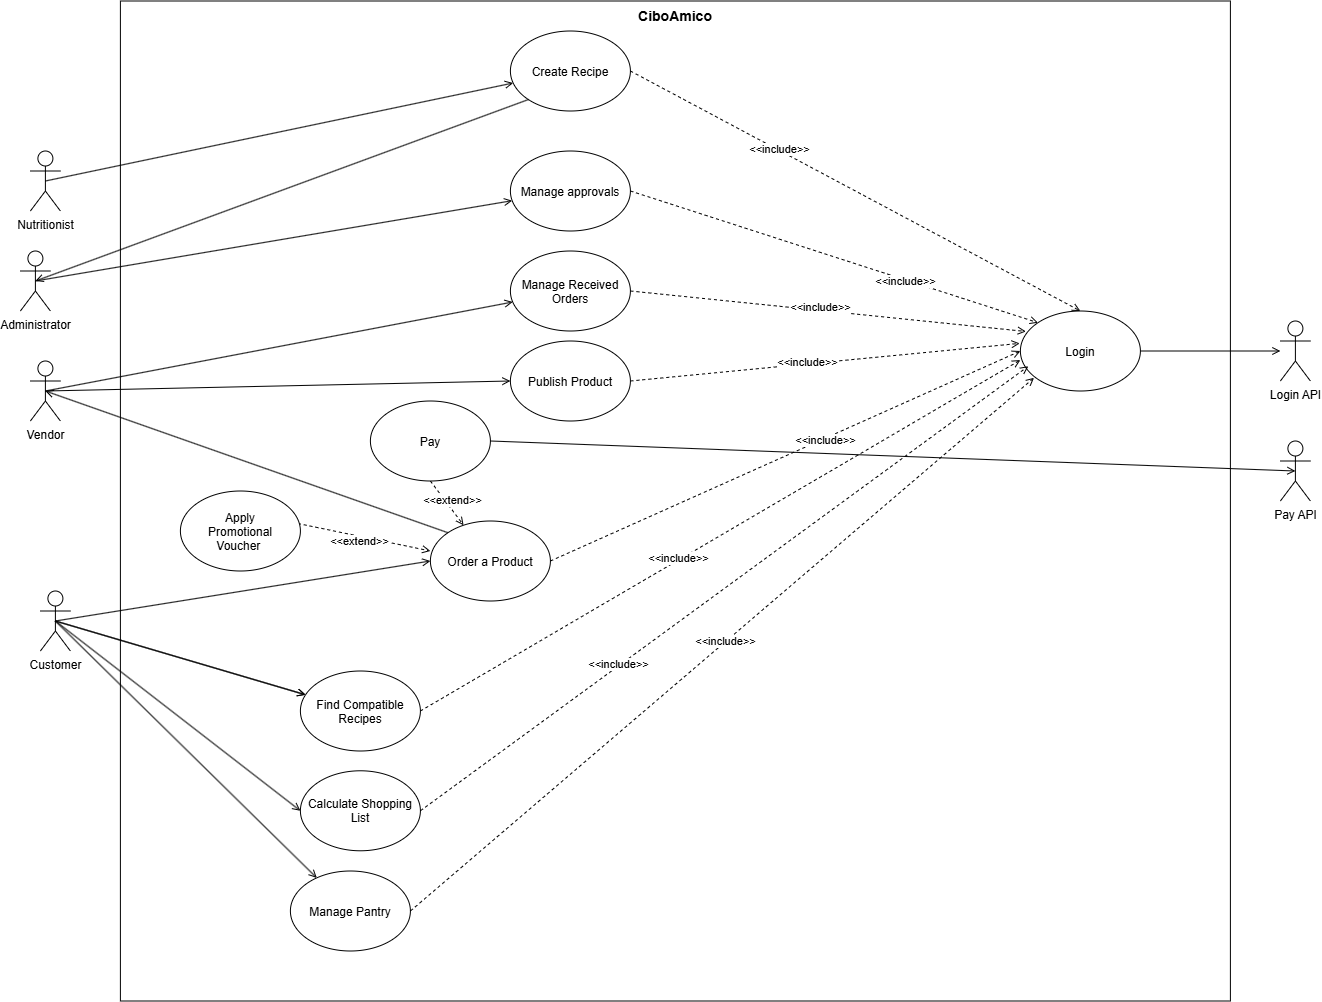
\includegraphics[width=0.95\textwidth]{figures/usecase_diagram_hr.png}
    \label{fig:usecase_diagram}
\end{figure}

\subsection{Internal Steps}
\label{subsec:uc_internal_steps}
\clearpage

\subsubsection{Order a Product}
\label{u:uc04}

\textbf{Main Flow:}
\begin{enumerate}
    \item The customer accesses the marketplace via Login.
    \item The system displays the available products with price and remaining stock.
    \item The customer selects a product from the catalog and starts the checkout.
    \item The system loads the selected product into the current order and computes the total amount.
    \item The customer confirms the purchase.
    \item The system requests the authorization for the debit of the computed amount from the Payment Service.
    \item The system registers the order in the ``CREATED'' state, decreases the remaining stock of the product and notifies the vendor.
\end{enumerate}

\textbf{Preconditions:} the customer is authenticated; at least one product is available in the catalog.

\textbf{Alternative Flow (Extensions):}
\begin{itemize}
    \item \textbf{3a. Product No Longer Available:} the selected product is not present in the catalog anymore; the system displays an error message.
    \item \textbf{4a. Promotional Voucher Request:} the customer requests to apply a promotional voucher to the current order; the system validates the temporal validity of the voucher and its association with the vendor of the selected product, recalculates the total amount applying the discount and resumes from step 5.
    \item \textbf{6a. Payment Rejected:} the Payment Service returns a negative outcome; the system cancels the current order and displays a failure message, returning the flow to step 4.
\end{itemize}
